\section{Materialverhalten}{}
    \subsection{Festigkeitshypothesen:}
        \subsubsection{Fliessbedingung:}
            Fliessfunktion: $\Phi(\sigma)$\\
            Fliessbedingung: $\Phi(\sigma)<0$ (elastisch), $\Phi(\sigma)=0$ (plastisch)
            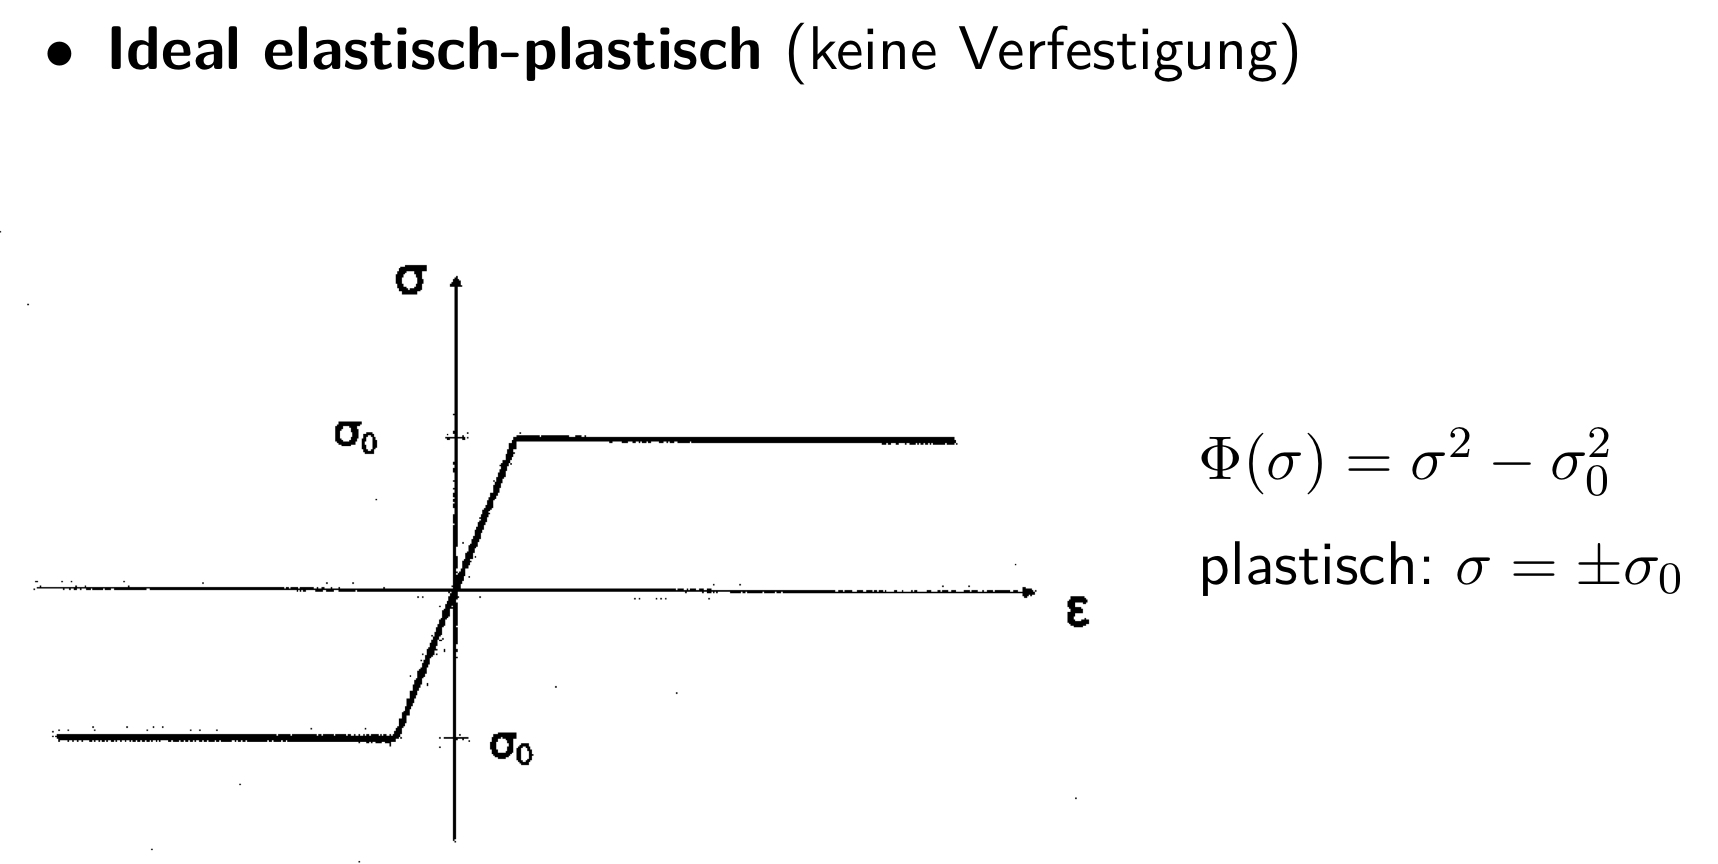
\includegraphics[width=0.45\linewidth]{04/Verf_ideal_elpl}
            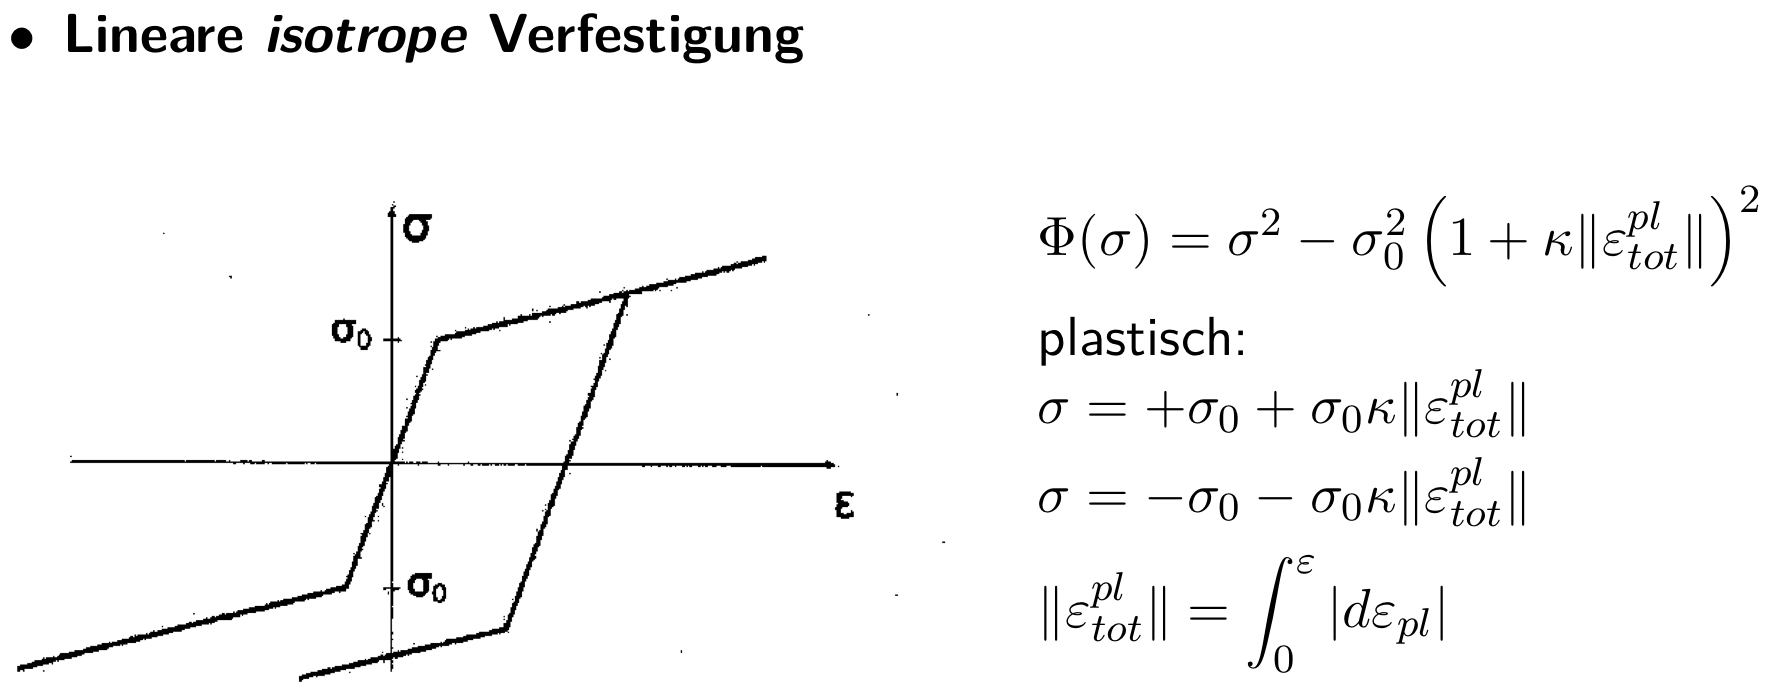
\includegraphics[width=0.5\linewidth]{04/Verf_lin_isotr}
            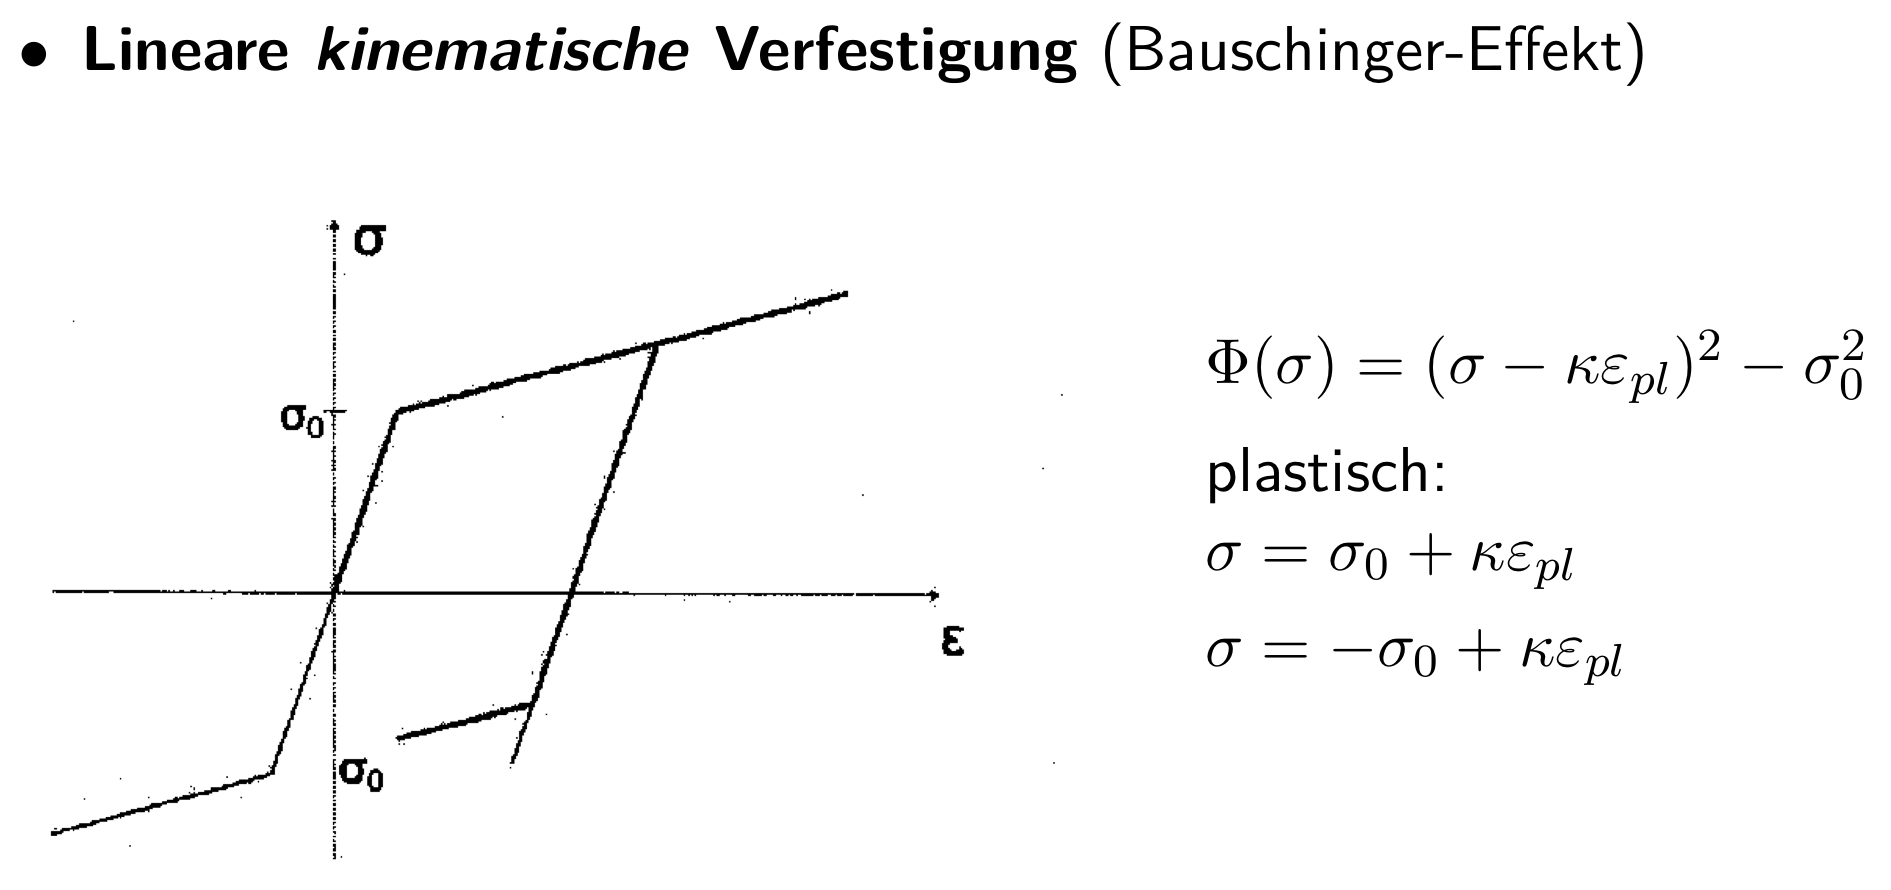
\includegraphics[width=0.5\linewidth]{04/Verf_lin_kin}
            
        \subsubsection{von Mieses'sche Vergleichsspannung:}
            \[\Phi_{v.Mises}= \sigma_1^2+\sigma_2^2+\sigma_3^2-\sigma_1\sigma_2-\sigma_1\sigma_3-\sigma_2\sigma_3 -\sigma_0^2\quad(=0)\]
            \[\Leftrightarrow \sigma_{v. Mises}^{vgl}= \sqrt{\sigma_1^2+\sigma_2^2+\sigma_3^2-\sigma_1\sigma_2-\sigma_1\sigma_3-\sigma_2\sigma_3} \quad\textrm(HS)\]
            
        \subsubsection{Tresca'sche Vergleichsspannung:}
            Konservativer als von Mises'sche Vergleichsspannung (Grenzfläche von Sechseck schneller erreicht als von Ellipse).
            \[\frac{1}{2}Max(|\sigma_1-\sigma_2|,|\sigma_2-\sigma_3|,|\sigma_3-\sigma_1|)=\tau_0=\frac{\sigma_0}{2}\]
        
        \subsubsection{Kesselgleichungen:}
            Für dünnwandige Behälter ($\frac{d}{R} \ll 1$)
            \[\sigma_{\varphi\varphi} = \frac{R}{d}P = 2\sigma_{zz}; \quad \sigma_{zz} = \frac{R}{2d}P; \quad \sigma_{rr}=0\]
            
    \subsection{Statische Belastung:}
        \begin{comment}
            \subsubsection{Kraft- \& Deformationsgesteurete Belastung:}
            $\frac{\epsilon_b}{\epsilon_0}$ Deformationsgesteurete Belastung. Bsp vorgespannte Schraube, therm Spannungen. Begrenzung weniger konservativ $\sigma\epsilon$-Diagramm gr Dehnung führt zu nur kl Spannungserhöhung).\\ $\frac{\sigma_B}{\sigma_0}$ Kraftgesteuerte Belastung. (Für viele Metalle $\frac{\epsilon_b}{\epsilon_0} \gg \frac{\sigma_B}{\sigma_0}$) Überschreiten $R_{p0.2}$ weniger Reserve.
        \end{comment}
        \subsubsection{Spannungsverteilung:}
            Falls homogen: bei Fliessgrenze wird die ganze Struktur plastifiziert.$\rightarrow$ Versagen %bei Erreichen der Fliessgrenze wird es in der ganzen Struktur zur Plastifizierung kommen. 
              
            Falls linear: es kommt an lokalen Stellen zu Plastifizierungen $\rightarrow$ Versagen erst bei einer grösseren Belastung.
        
      
      Zug:
            Erste plastifizierung = vollständige Plastifizierung:
        
            $F_{plast} = \sigma_0\ * A$
            
      Biegung:
            Erste Plastifizierung:
            
            $M_{plast} = \sigma_0*I*\frac{1}{d}$
            
           $M_{versagen} = 2$ $\int_{-b/2}^{b/2}\int_{0}^{h/2}\sigma(y)ydydz$ mit $\sigma(y) = \sigma_0$
            
            
        \subsubsection{Formfaktoren:}
        
            Zug(homogen): $\frac{F_{versagen}}{F_{plast}}$
            
            Biegung(linear):
            $\frac{P_{versagen}}{P_{plast}}$